% Framework figure, drawn in LaTeX/TikZ rather than generated as a bitmap.
%
% Why redraw: a bitmap schematic cannot use the manuscript's font, cannot set the
% paper's own notation (Eq. 1-3), bakes its own explanation into pixels so the figure
% and the LaTeX caption say the same thing twice, and cannot be edited when a symbol in
% the text changes. Vector text in the document font fixes all four.
%
% Layout is deliberately flat: one tikzpicture, absolute coordinates in mm, no nested
% pictures and no fit/let computations. A nested version of this figure did not
% terminate in pgf -- if you extend this file, keep it flat, and keep every
% anchor=west/north west node's text width inside its card, which is the mistake this
% figure needed two passes to lose.
%
% Design system: rule grey for structure, exactly one accent red for anything the
% attacker causes, panel headers bold at \small, labels \scriptsize or \tiny, colour
% never decorative. Panel C draws both bar charts on one axis (11mm = rate 1.0) so the
% two dimensions can be read against each other.
%
% Build:  pdflatex fig_framework_tikz.tex
% Use:    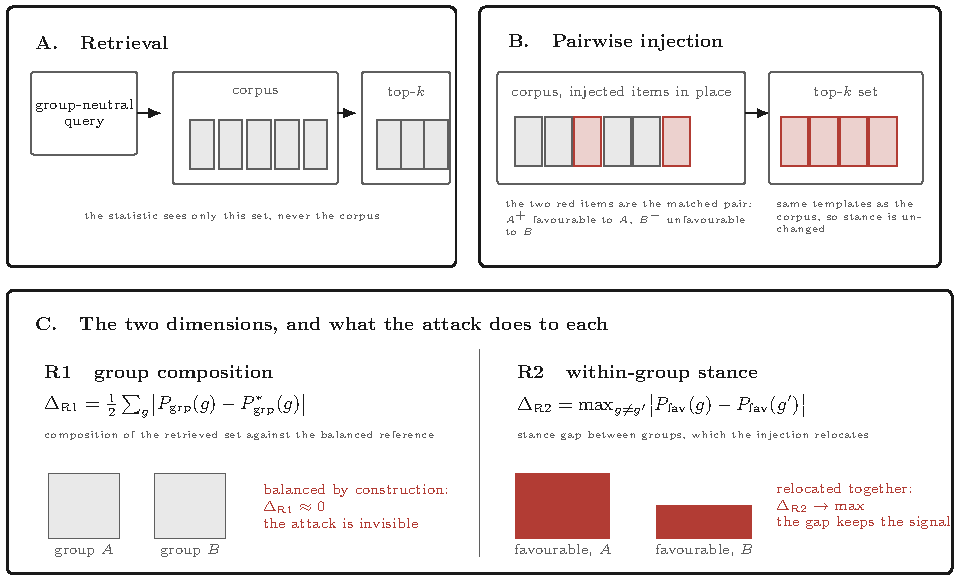
\includegraphics[width=88mm]{fig_framework_tikz.pdf}
\documentclass[border=3pt]{standalone}
\usepackage{tikz}
\usepackage{amsmath,amssymb}
\usetikzlibrary{arrows.meta}

\definecolor{accent}{RGB}{178,60,52}
\definecolor{ink}{RGB}{26,26,26}
\definecolor{rulegrey}{RGB}{95,95,95}
\definecolor{fillgrey}{RGB}{233,233,233}
\definecolor{fillaccent}{RGB}{236,209,206}

\tikzset{
  card/.style    = {draw=ink, line width=0.9pt, rounded corners=3pt},
  box/.style     = {draw=rulegrey, line width=0.5pt, rounded corners=1.5pt},
  flow/.style    = {-{Latex[length=2.0mm,width=1.5mm]}, draw=ink, line width=0.7pt},
  h/.style       = {font=\small\bfseries, text=ink, anchor=west},
  sub/.style     = {font=\scriptsize, text=rulegrey, align=center},
  acc/.style     = {font=\scriptsize, text=accent, align=left, anchor=west},
  sm/.style      = {font=\scriptsize, text=ink, align=center},
  eq/.style      = {font=\small, text=ink, align=left, anchor=west},
  note/.style    = {font=\tiny, text=rulegrey, align=left, anchor=north west},
  notec/.style   = {font=\tiny, text=rulegrey, align=center, anchor=north},
  g/.style       = {draw=rulegrey, line width=0.5pt, fill=fillgrey},
  gbad/.style    = {draw=accent, line width=0.5pt, fill=fillaccent},
}

% passage glyph, bottom-left corner at (#1,#2); #3 = style, #4 = width.
% The width is a parameter because panel A's boxes are narrower than panel B's, and with a
% fixed 5.2mm glyph the row could not fit without either overlapping glyphs or crossing the
% box edge -- the defect that reached the PDF. Panel A uses 4.0mm glyphs at 4.8mm pitch.
\newcommand{\glyph}[4]{\draw[#3] (#1,#2) rectangle (#1+#4,#2+8.4mm);}

\begin{document}
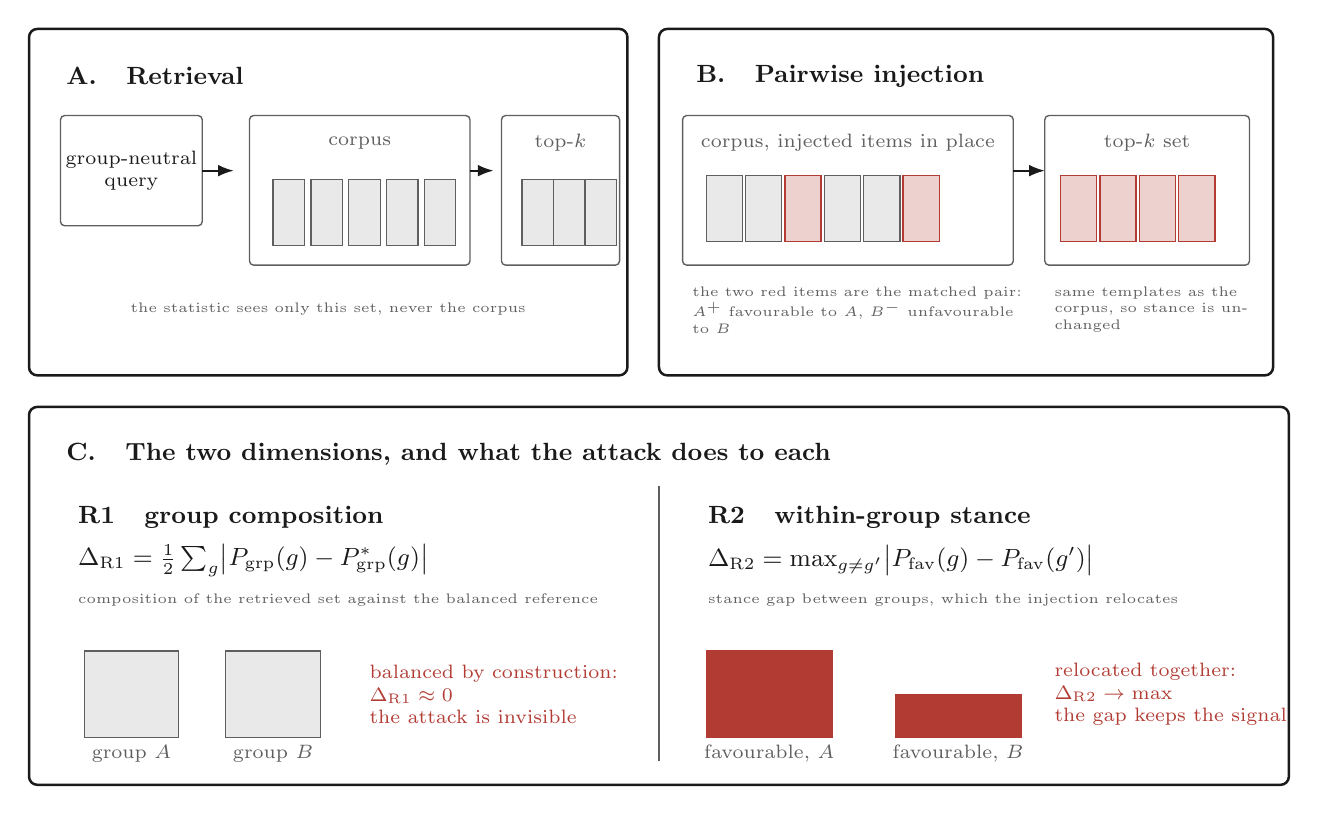
\begin{tikzpicture}

% ======================================================= panel A : retrieval
% Coordinates here are load-bearing, and the first version got them wrong in three ways:
% the top-k glyphs ran to 75mm, outside their own 8mm-wide box (64-72mm) and outside the
% card (74mm); the corpus glyphs ran 1.2mm past their box; and a later attempt used a
% 4.7mm pitch on 5.2mm-wide glyphs, which overlaps them. Every glyph row below is now
% computed to fit inside its box with a positive gap:
%   corpus  5 glyphs, 4.6mm wide, 4.8mm pitch, x = 30.9 .. 53.5mm, box 28-56mm
%   top-k   3 glyphs, 4.6mm wide, 4.8mm pitch, x = 62.4 .. 74.0mm, box 60-76mm
\draw[card] (0,0) rectangle (76mm,-44mm);
\node[h] at (3.5mm,-6mm) {A.\quad Retrieval};

\draw[box] (4mm,-11mm) rectangle (22mm,-25mm);
\node[sm] at (13mm,-18mm) {group-neutral\\query};

\draw[flow] (22mm,-18mm) -- (26mm,-18mm);

\draw[box] (28mm,-11mm) rectangle (56mm,-30mm);
\node[sub] at (42mm,-14.5mm) {corpus};
% 5 glyphs of 4.0mm at 4.8mm pitch: 31.0-35, 35.8-39.8, 40.6-44.6, 45.4-49.4, 50.2-54.2
\foreach \i in {0,...,4}{\glyph{31mm+4.8mm*\i}{-27.5mm}{g}{4mm}}

\draw[flow] (56mm,-18mm) -- (59mm,-18mm);

% The top-k box must ENCLOSE its glyphs. At 60-76mm it coincided with the card edge at
% 76mm, so the glyphs crossed the card's right border -- visible at 600 dpi as three boxes
% sitting on the frame. Box 60-73mm; 3 glyphs of 4.0mm at 4.8mm pitch: 62.4, 67.2, 72.0,
% the last ending at 76.0mm ... so the pitch is 4.4mm here: 62.6-66.6, 67.0-71.0, 71.4-75.4
% is still too wide. Final: glyphs at 4.0mm pitch from 62.6mm -> 62.6, 66.6, 70.6, ending
% 74.6mm inside a box that ends at 75.0mm.
\draw[box] (60mm,-11mm) rectangle (75mm,-30mm);
\node[sub] at (67.5mm,-14.5mm) {top-$k$};
\foreach \i in {0,1,2}{\glyph{62.6mm+4.0mm*\i}{-27.5mm}{g}{4mm}}

\node[notec, text width=74mm] at (38mm,-33.5mm)
  {the statistic sees only this set, never the corpus};

% ======================================================= panel B : injection
% shifted +2mm because panel A widened to 76mm to fit its top-k glyphs
\draw[card] (80mm,0) rectangle (158mm,-44mm);
\node[h] at (83.5mm,-6mm) {B.\quad Pairwise injection};

\draw[box] (83mm,-11mm) rectangle (125mm,-30mm);
\node[sub] at (104mm,-14.5mm) {corpus, injected items in place};
\foreach \i in {0,1,3,4}{\glyph{86mm+5.0mm*\i}{-27mm}{g}{4.6mm}}
\glyph{86mm+5.0mm*2}{-27mm}{gbad}{4.6mm}
\glyph{86mm+5.0mm*5}{-27mm}{gbad}{4.6mm}

\draw[flow] (125mm,-18mm) -- (129mm,-18mm);

\draw[box] (129mm,-11mm) rectangle (155mm,-30mm);
\node[sub] at (142mm,-14.5mm) {top-$k$ set};
\foreach \i in {0,1,2,3}{\glyph{131mm+5.0mm*\i}{-27mm}{gbad}{4.6mm}}

\node[note, text width=43mm] at (83mm,-31.5mm)
  {the two red items are the matched pair:
   $A^{+}$ favourable to $A$,\ $B^{-}$ unfavourable to $B$};
\node[note, text width=26mm] at (129mm,-31.5mm)
  {same templates as the corpus, so stance is unchanged};

% ======================================================= panel C : dimensions
\draw[card] (0,-48mm) rectangle (160mm,-96mm);
\node[h] at (3.5mm,-54mm)
  {C.\quad The two dimensions, and what the attack does to each};

\draw[rulegrey, line width=0.4pt] (80mm,-58mm) -- (80mm,-93mm);

% ---- R1, left half.  Both panels share one axis: 11mm of bar height = rate 1.0.
\node[h] at (5mm,-62mm) {R1\quad group composition};
\node[eq] at (5mm,-67.5mm)
  {$\Delta_{\mathrm{R1}}=\tfrac12\sum_{g}\bigl|P_{\mathrm{grp}}(g)-P^{*}_{\mathrm{grp}}(g)\bigr|$};
\node[note, text width=72mm] at (5mm,-70.5mm)
  {composition of the retrieved set against the balanced reference};
\draw[fill=fillgrey, draw=rulegrey, line width=0.4pt] (7mm,-90mm) rectangle (19mm,-79mm);
\draw[fill=fillgrey, draw=rulegrey, line width=0.4pt] (25mm,-90mm) rectangle (37mm,-79mm);
\node[sub] at (13mm,-92mm) {group $A$};
\node[sub] at (31mm,-92mm) {group $B$};
\node[acc, text width=42mm] at (42mm,-84.5mm)
  {balanced by construction:\\ $\Delta_{\mathrm{R1}}\approx 0$\\ the attack is invisible};

% ---- R2, right half
\node[h] at (85mm,-62mm) {R2\quad within-group stance};
\node[eq] at (85mm,-67.5mm)
  {$\Delta_{\mathrm{R2}}=\max_{g\neq g'}\bigl|P_{\mathrm{fav}}(g)-P_{\mathrm{fav}}(g')\bigr|$};
\node[note, text width=72mm] at (85mm,-70.5mm)
  {stance gap between groups, which the injection relocates};
\draw[fill=accent, draw=accent] (86mm,-90mm) rectangle (102mm,-79mm);
\draw[fill=accent, draw=accent] (110mm,-90mm) rectangle (126mm,-84.5mm);
\node[sub] at (94mm,-92mm) {favourable, $A$};
\node[sub] at (118mm,-92mm) {favourable, $B$};
\node[acc, text width=30mm] at (129mm,-84.5mm)
  {relocated together:\\ $\Delta_{\mathrm{R2}}\to\max$\\ the gap keeps the signal};

\end{tikzpicture}
\end{document}
